\documentclass[11pt,a4paper]{article}
\usepackage[T1]{fontenc}
\usepackage{amsmath}
\usepackage{graphicx}
\usepackage{hyperref}
\usepackage{longtable}
\usepackage{geometry}
\geometry{margin=25mm}
\title{Atmospheric Simulation}
\author{Simulation Team}
\date{28 September 2026}
\begin{document}
\maketitle
\begin{center}\large A Brief++ feature tour\end{center}
\begin{center}Example Research Lab\end{center}
\begin{abstract}
A small, self-contained report showing the document model and all seven output formats.
\end{abstract}
\section{Introduction and scope}\label{introduction}
\begin{quote}
This report combines \textbf{measurements} with an \emph{idealized} model. The word \texttt{Brief++} refers to the report builder. See the \href{https://github.com/vrtulka23/briefpp}{project source} for the code and \ref{density-profile} for the generated figure. The report builder is documented by \cite{example2026}.

\end{quote}
\begin{quote}
A report should preserve the meaning of its content across formats.
\end{quote}
\begin{quote}\textbf{note:} The numbers below are illustrative rather than observational data.\end{quote}
\section{Model}\label{model}
The pressure model uses a scale height \(H = 8.4\,\mathrm{km}\) under a constant-temperature assumption.

\begin{equation}
\frac{dP}{dz} = -\rho g
\label{hydrostatic}
\end{equation}
\begin{equation}
P(z) = P_0 e^{-z/H}
\label{pressure-profile}
\end{equation}
Equation \ref{pressure-profile} describes the synthetic curve used here.

\begin{verbatim}
double pressure(double z, double p0, double h) {
    return p0 * std::exp(-z / h);
}
\end{verbatim}
\section{Results}\label{results}
\begin{figure}[htbp]
\centering
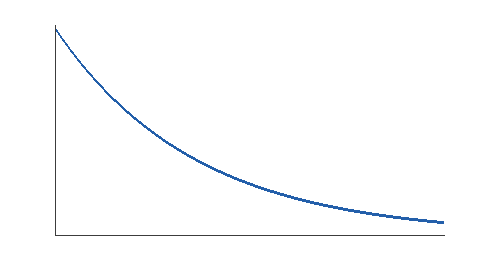
\includegraphics[width=0.8\linewidth]{density.png}
\caption{Synthetic atmospheric \textbf{density} by altitude.}
\label{density-profile}
\end{figure}
\begin{longtable}{lll}
\caption{Illustrative sea-level conditions}\label{conditions}\\
Parameter & Value & Unit \\
\hline
Temperature & 273.15 & K \\
Pressure & 101325 & Pa \\
\textbf{Scale height} & 8.4 & km \\
\end{longtable}
The values in \ref{conditions} produce the trend shown in \ref{density-profile}.

\begin{enumerate}
\item Set the starting conditions
\item Review the output in every format
\item Compare the rendered documents
\end{enumerate}
\begin{itemize}
\item \textbf{Check the details}
\begin{itemize}
\item Check the figure and table
\item Check the linked references
\end{itemize}
\end{itemize}
\begin{description}
\item[Density] Mass per unit volume
\item[\textbf{Scale height}] Altitude over which pressure falls by a factor of \(e\).
\end{description}
\subsection{Interpretation}
The example emphasizes report structure, not atmospheric accuracy.

\begin{quote}\textbf{warning:} Do not use these illustrative values for a real forecast.\end{quote}
\begin{quote}\textbf{tip:} Edit this source file and rebuild the demo to compare formats.\end{quote}
\par\noindent\rule{\linewidth}{0.4pt}\par
\begin{longtable}{ll}
\caption{Headerless summary table}\\
Input & Illustrative profile \\
Outputs & Seven text formats and a PDF \\
\end{longtable}
This paragraph was added from a \texttt{DocumentFragment} to demonstrate reusable content.

\newpage
\section{Backend-specific notes}
\noindent\textit{LaTeX-only note.}
\begin{thebibliography}{9}
\bibitem{example2026} Brief++ contributors. Brief++ project source and documentation. 2026. \url{https://github.com/vrtulka23/briefpp}
\end{thebibliography}
\end{document}
